\documentclass[tikz,border=5pt]{standalone}
\usepackage[T1]{fontenc}
\usepackage{lmodern,amsmath,amssymb}
\usetikzlibrary{arrows.meta,calc,positioning,fit,backgrounds,shapes.geometric,matrix,decorations.pathreplacing,patterns}
\definecolor{ink}{gray}{0.08}
\definecolor{wash}{gray}{0.965}
\definecolor{soft}{gray}{0.45}
\tikzset{box/.style={draw=ink,line width=.65pt,fill=white,align=center,inner sep=4pt,outer sep=0pt,font=\small},flow/.style={draw=ink,line width=.65pt,-{Latex[length=1.8mm,width=1.3mm]},rounded corners=2pt},annotation/.style={font=\scriptsize,text=soft,align=center},groupbox/.style={draw=soft,dashed,line width=.45pt,fill=wash}}
\begin{document}
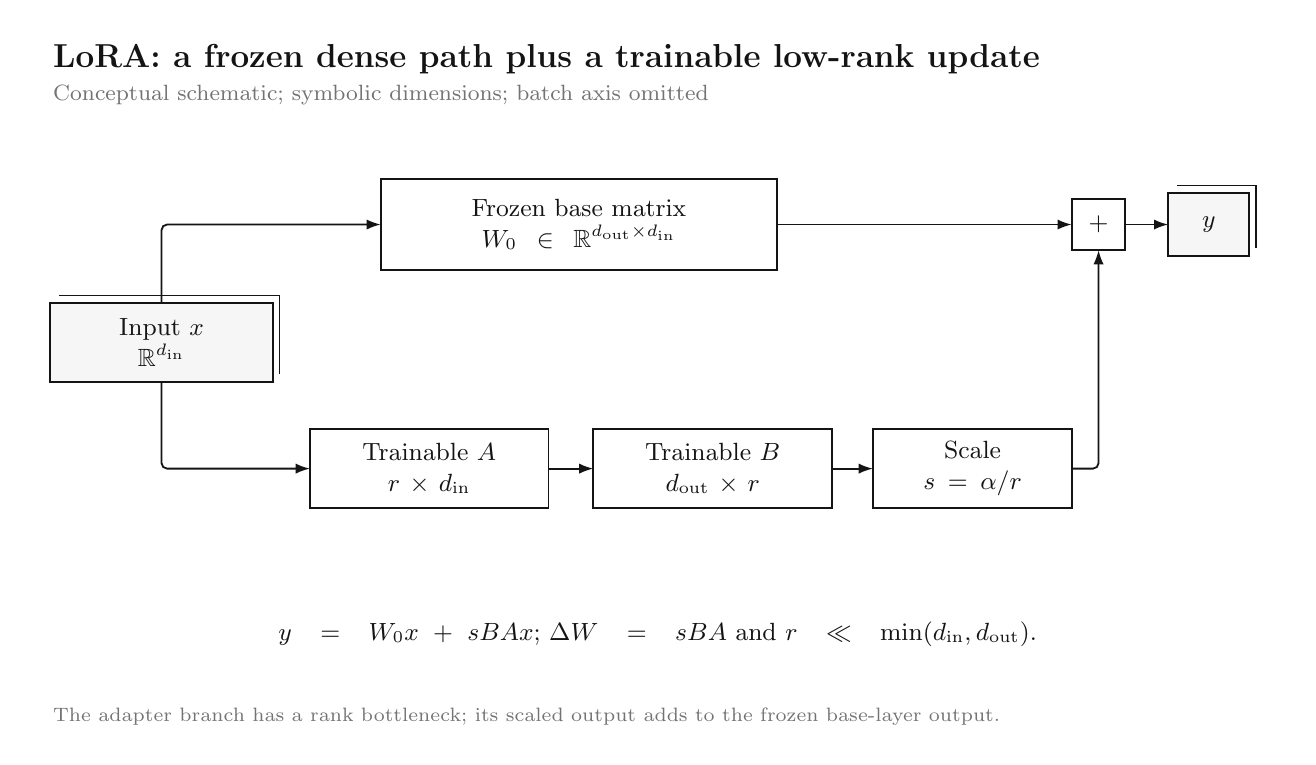
\begin{tikzpicture}[x=1cm,y=-1cm,font=\rmfamily,text=ink]

\path[use as bounding box] (0,0) rectangle (16,9);
\node[anchor=west,font=\large\bfseries] at (.2,.4) {LoRA: a frozen dense path plus a trainable low-rank update};
\node[anchor=west,font=\footnotesize,text=soft] at (.2,.85) {Conceptual schematic; symbolic dimensions; batch axis omitted};
\begin{pgfonlayer}{background}
\end{pgfonlayer}
\node[box,fill=wash,minimum width=2.8cm,minimum height=1.0cm,text width=2.55cm] (x) at (1.7,4.0) {Input $x$\\$\mathbb{R}^{d_{\rm in}}$};
\draw[ink,line width=.4pt] (0.4,3.4) -- (3.1999999999999997,3.4) -- (3.1999999999999997,4.4);
\node[box,minimum width=5.0cm,minimum height=1.15cm,text width=4.75cm] (base) at (7.0,2.5) {Frozen base matrix\\$W_0\in\mathbb{R}^{d_{\rm out}\times d_{\rm in}}$};
\node[box,minimum width=3.0cm,minimum height=1.0cm,text width=2.75cm] (a) at (5.1,5.6) {Trainable $A$\\$r\times d_{\rm in}$};
\node[box,minimum width=3.0cm,minimum height=1.0cm,text width=2.75cm] (b) at (8.7,5.6) {Trainable $B$\\$d_{\rm out}\times r$};
\node[box,minimum width=2.5cm,minimum height=1.0cm,text width=2.25cm] (scale) at (12,5.6) {Scale\\$s=\alpha/r$};
\node[box,minimum width=0.65cm,minimum height=0.65cm,text width=0.4cm] (add) at (13.6,2.5) {$+$};
\node[box,fill=wash,minimum width=1.0cm,minimum height=0.8cm,text width=0.75cm] (out) at (15,2.5) {$y$};
\draw[ink,line width=.4pt] (14.6,2.0) -- (15.6,2.0) -- (15.6,2.8);
\node[align=center,inner sep=0pt,outer sep=0pt,font=\small,minimum width=13.8cm,minimum height=0.7cm,text width=13.55cm] (note7) at (8,7.7) {$y=W_0x+sBAx$; $\Delta W=sBA$ and $r\ll\min(d_{\rm in},d_{\rm out})$.};
\begin{pgfonlayer}{background}
\draw[flow] (x.north) -- (1.7,2.5) -- (base.west);
\draw[flow] (x.south) -- (1.7,5.6) -- (a.west);
\draw[flow] (base.east) -- (add.west);
\draw[flow] (a.east) -- (b.west);
\draw[flow] (b.east) -- (scale.west);
\draw[flow] (scale.east) -- (13.6,5.6) -- (add.south);
\draw[flow] (add.east) -- (out.west);
\end{pgfonlayer}
\node[anchor=west,align=left,font=\scriptsize,text=soft,text width=15.6cm] at (.2,8.75) {The adapter branch has a rank bottleneck; its scaled output adds to the frozen base-layer output.};
\end{tikzpicture}
\end{document}
